\documentclass[11pt,aspectratio=169]{beamer}
\usepackage{amsmath,amssymb,bm,graphicx,booktabs,tikz,pgfplots}
\pgfplotsset{compat=1.17}
\usetikzlibrary{arrows.meta,positioning}

\usetheme{default}
\setbeamertemplate{navigation symbols}{}
\setbeamertemplate{headline}{}
\setbeamertemplate{footline}{%
  \leavevmode
  \hbox{%
    \begin{beamercolorbox}[wd=\paperwidth,ht=2.6ex,dp=1.1ex,right]{page number in head/foot}%
      \insertframenumber/\inserttotalframenumber\hspace{0.35cm}
    \end{beamercolorbox}%
  }%
}
\setbeamertemplate{frametitle}{\vspace{0.25cm}\insertframetitle\par\vspace{0.08cm}\hrule}
\setbeamercolor{normal text}{fg=black,bg=white}
\setbeamercolor{frametitle}{fg=black,bg=white}
\setbeamercolor{structure}{fg=black}
\setbeamersize{text margin left=0.7cm,text margin right=0.7cm}

\newcommand{\dd}{\,\mathrm{d}}
\newcommand{\Om}{\Omega}
\newcommand{\Gam}{\Gamma}
\newcommand{\R}{\mathbb R}
\newcommand{\Th}{\mathcal T_h}
\newcommand{\Vzero}{\mathcal V_0}
\newcommand{\Vhzero}{\mathcal V_{h,0}}
\newcommand{\Ih}{\mathcal I_h}
\newcommand{\Ie}{\mathcal I_e}
\newcommand{\norm}[2][]{\left\lVert#2\right\rVert_{#1}}
\newcommand{\seminorm}[2][]{\left\lvert#2\right\rvert_{#1}}
\newcommand{\bx}{\bm x}
\newcommand{\bu}{\bm u}
\newcommand{\bv}{\bm v}
\newcommand{\beps}{\bm\varepsilon}

% Frozen output of Chapter 7, Example 7.5, copied here for reproducibility.
\graphicspath{{figures/}}

\begin{document}

\begin{frame}[plain]
  \centering\vfill
  {\LARGE\bfseries A Priori Error Analysis\par}
  \vspace{0.45cm}
  {\large Interpolation estimates and finite element error bounds\par}
  \vfill
\end{frame}

\begin{frame}{Lecture outline}
This lecture begins where the previous lecture stopped: after the proof of
C\'ea's lemma.

\begin{enumerate}
  \item Construct the nodal interpolant and prove the interpolation estimates
  for linear elements in one dimension.
  \item State the corresponding result on shape-regular triangular and
  tetrahedral meshes.
  \item Combine interpolation with the energy best-approximation property to
  obtain finite element error estimates.
\end{enumerate}

The optimal $L^2$ estimate requires an additional duality argument and is the
first main topic of the next lecture.
\end{frame}

\section{Finite element interpolation}

\begin{frame}[plain]
  \centering
  \vfill
  {\LARGE\bfseries Finite element interpolation\par}
  \vspace{0.45cm}
  {\large Construct a finite element function from the nodal values of a
  given function.\par}
  \vfill
\end{frame}

\begin{frame}{Finite element interpolant}
To use C\'ea's lemma, we need a specific function $v_h\in V_h$ whose error
can be estimated. We choose the nodal interpolant.

Let $V_h$ be a Lagrange finite element space with global nodes $\bx_i$ and
nodal basis functions $\phi_i$. For a continuous function $u$, define
\[
  \boxed{
  \Ih u
  =\sum_{i=1}^{N_n}u(\bx_i)\phi_i.}
\]
The interpolant belongs to $V_h$ and satisfies
\[
  \Ih u(\bx_i)=u(\bx_i)
  \qquad i=1,\ldots,N_n.
\]

On an element $\mathcal K_e$,
\[
  (\Ih u)|_{\mathcal K_e}
  =\Ie(u|_{\mathcal K_e}).
\]
Thus the global interpolant can be constructed cell by cell from the nodal
values of $u$.
\end{frame}

\begin{frame}{Interpolation on a triangular mesh}
  \centering
  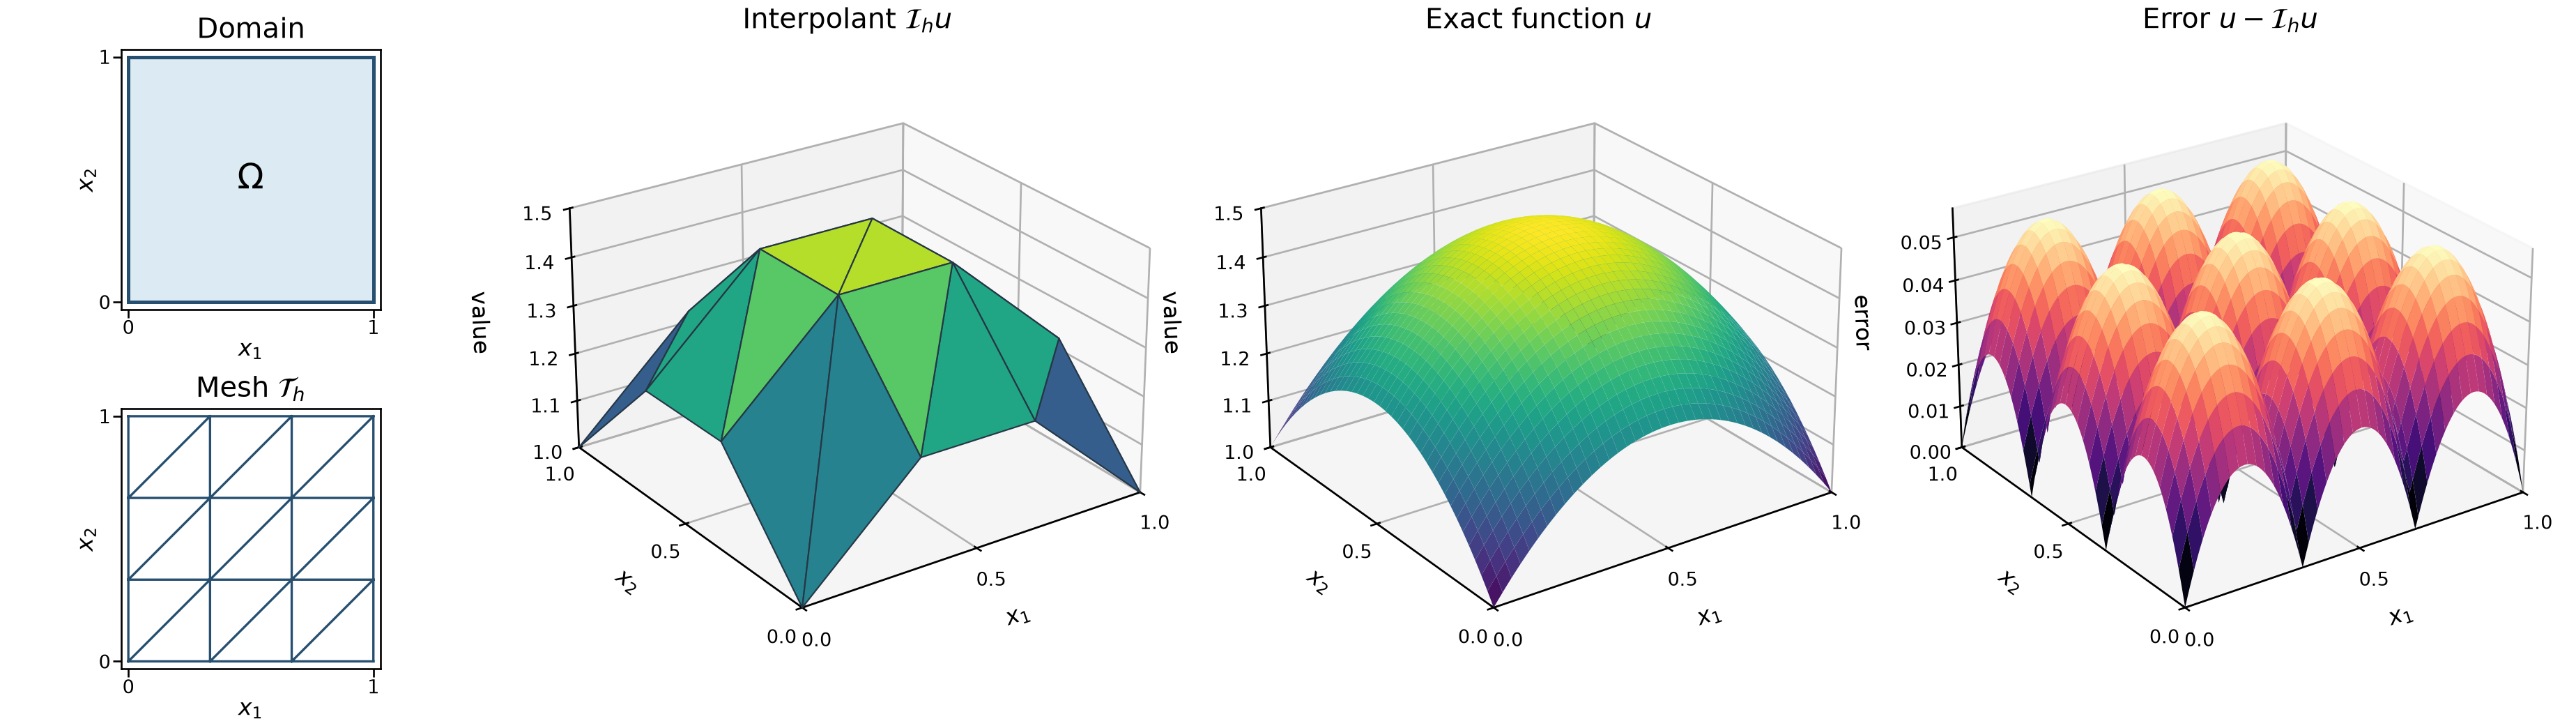
\includegraphics[width=0.99\textwidth]{c7_interpolation_2d.png}

  \vspace{0.05cm}
  The coarse mesh defines the $P_1$ interpolant. The finer plotting points
  only display the exact function and the error smoothly; they are not
  additional finite element nodes. For this quadratic and uniform mesh, the
  error pattern repeats on every triangle up to translation or reflection.
\end{frame}

\begin{frame}{Interpolation after uniform refinement}
  \centering
  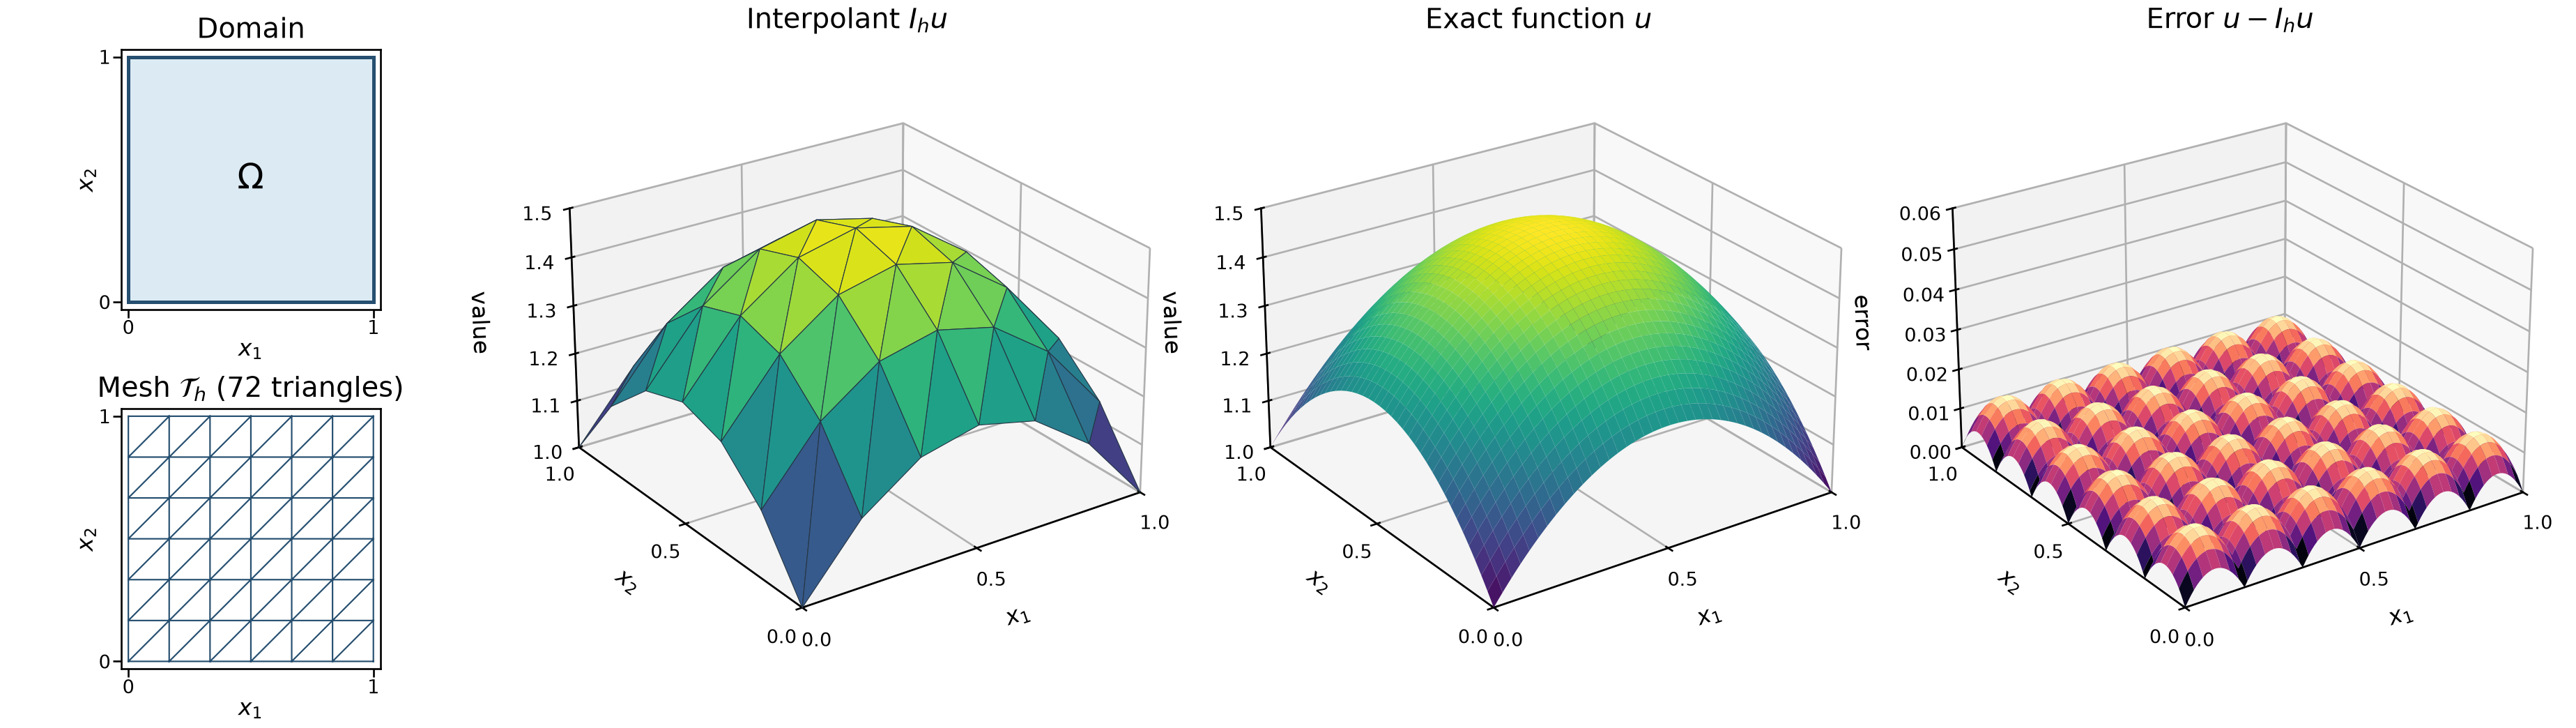
\includegraphics[width=0.99\textwidth]{c7_interpolation_2d_fine.png}

  \vspace{0.05cm}
  Halving the grid spacing increases the mesh from 18 to 72 triangles. With
  the same vertical scales in both figures, the maximum error decreases from
  $1/18$ to $1/72$, a factor of four.
\end{frame}

\begin{frame}{Properties and regularity of the interpolant}
Three properties will be used in the error estimates.
\begin{enumerate}
  \item \textbf{Locality:} $(\Ih u)|_{\mathcal K_e}$ depends only on
  the degrees of freedom of $\mathcal K_e$.
  \item \textbf{Polynomial reproduction:} if
  $u|_{\mathcal K_e}$ belongs to the local finite element space, then
  $\Ie u=u$ on $\mathcal K_e$.
  \item \textbf{Boundary values:} if $u=0$ on $\Gam_D$ and the mesh resolves
  $\Gam_D$, then $\Ih u\in\Vhzero$.
\end{enumerate}

\vspace{0.2cm}
The nodal interpolant requires point values. In one dimension, $H^1$
functions are continuous. In two and three dimensions, a general $H^1$
function need not be continuous, so the estimates will assume additional
regularity, commonly $u\in H^2(\Om)$.
\end{frame}

\section{Linear interpolation in one dimension}

\begin{frame}{A four-element linear mesh}
Consider $u(x)=1+x(1-x)$ on $[0,1]$. Use four uniform linear elements with
five nodes:
\[
  x_1=0,
  \qquad x_2=\frac14,
  \qquad x_3=\frac12,
  \qquad x_4=\frac34,
  \qquad x_5=1.
\]

On $\mathcal K_e=[x_e,x_{e+1}]$,
\[
  \Ie u
  =u(x_e)\phi_1^e+u(x_{e+1})\phi_2^e.
\]

The interpolant agrees with $u$ at both element nodes and is linear between
them. Adjacent local interpolants share the same value at their common node,
so the global interpolant is continuous.
\end{frame}

\begin{frame}{Exact function, interpolant, and error}
  \centering
  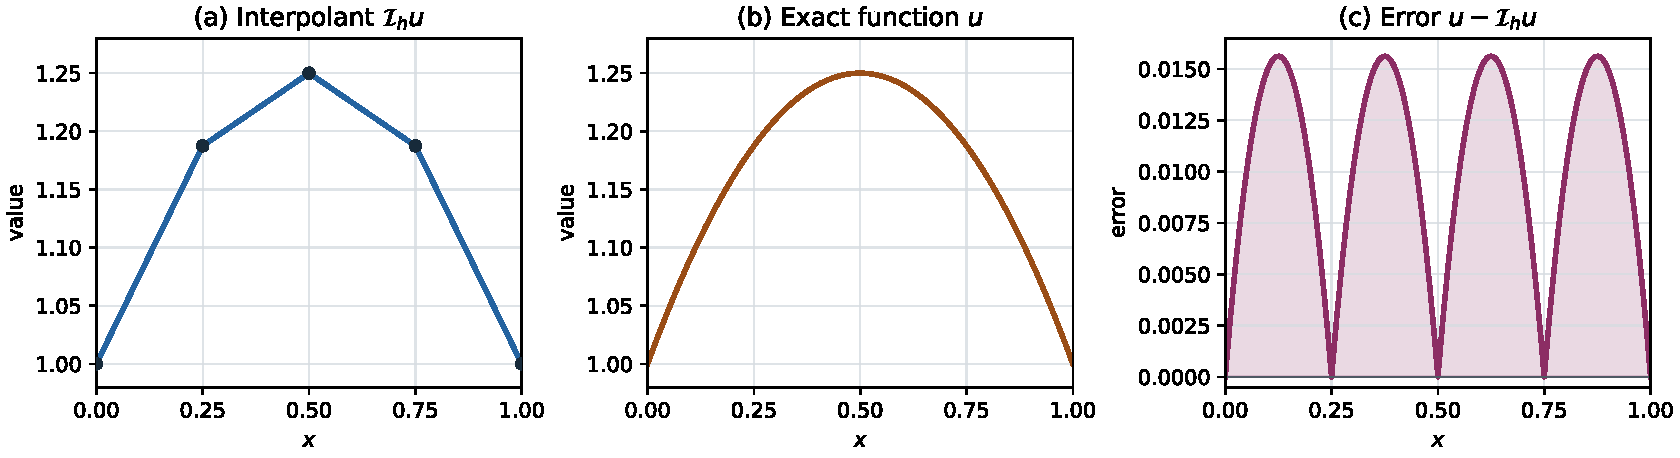
\includegraphics[width=0.96\textwidth]{c7_interpolation_1d.pdf}

  \vspace{0.08cm}
  On every element,
  \[
    u(x)-\Ie u(x)
    =(x-x_e)(x_{e+1}-x).
  \]
  Since $h=1/4$ on each element, the error reaches the same maximum
  $h^2/4=1/64$ at every element midpoint.
\end{frame}

\begin{frame}{Interpolation on eight linear elements}
  \centering
  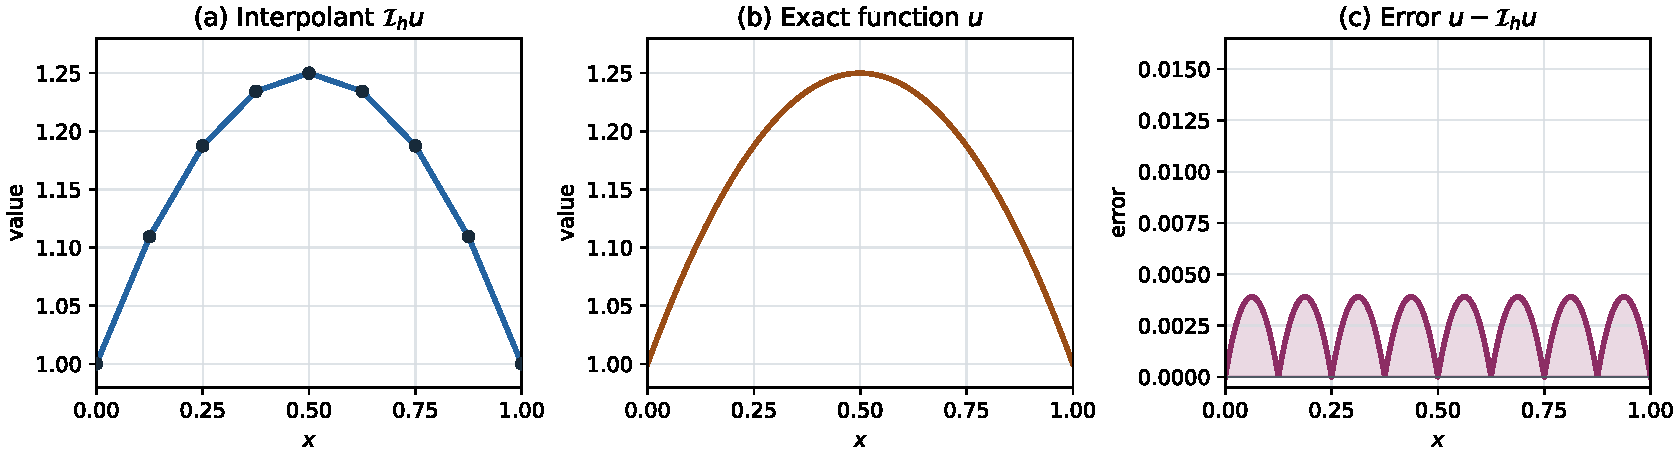
\includegraphics[width=0.96\textwidth]{c7_interpolation_1d_fine.pdf}

  \vspace{0.08cm}
  Dividing every coarse element in two gives nine nodes
  $x_i=(i-1)/8$. The element length decreases from $1/4$ to $1/8$, and the
  maximum error decreases from $1/64$ to $1/256$.
\end{frame}

\begin{frame}[plain]
  \centering
  \vfill
  {\LARGE\bfseries Interpolation estimates in one dimension\par}
  \vspace{0.45cm}
  {\large Estimate the error on one element, then sum the element estimates
  over the mesh.\par}
  \vfill
\end{frame}

\begin{frame}{Local interpolation estimates}
Let $\mathcal K_e=(x_e,x_{e+1})$, $h_e=x_{e+1}-x_e$, and
$u\in H^2(\mathcal K_e)$. Then
\[
  \boxed{
  \norm[L^2(\mathcal K_e)]{(u-\Ie u)'}
  \leq
  h_e\norm[L^2(\mathcal K_e)]{u''}}
\]
and
\[
  \boxed{
  \norm[L^2(\mathcal K_e)]{u-\Ie u}
  \leq
  h_e^2\norm[L^2(\mathcal K_e)]{u''}.}
\]

The derivative error contains one power of $h_e$. The error in the function
values contains two powers of $h_e$.
\end{frame}

\begin{frame}{Why the derivative error vanishes at one point}
Set
\[
  w=u-\Ie u.
\]
Because $\Ie u$ is linear, $w''=u''$. Also,
\[
  w(x_e)=w(x_{e+1})=0.
\]

\textbf{Rolle's theorem.} If a function is continuous on $[a,b]$,
differentiable on $(a,b)$, and has equal endpoint values, then its derivative
is zero at some point in $(a,b)$.

In one dimension, an $H^2$ function has a continuously differentiable
representative. Rolle's theorem therefore gives
\[
  x_*\in(x_e,x_{e+1})
  \qquad\text{such that}\qquad
  w'(x_*)=0.
\]
The fundamental theorem of calculus, applied to $w'$, now gives
\[
  w'(y)-w'(x_*)=\int_{x_*}^{y}w''(t)\,\dd t,
  \qquad
  w'(y)=\int_{x_*}^{y}w''(t)\,\dd t.
\]
\end{frame}

\begin{frame}{The pointwise derivative bound}
For $y\in\mathcal K_e$, let $I_y$ be the interval with endpoints $x_*$ and
$y$. Its length satisfies $|I_y|\leq h_e$. Therefore
\begin{align*}
  |w'(y)|^2
  &=
  \left|\int_{I_y}1\,w''(t)\,\dd t\right|^2\\
  &\leq
  \left(\int_{I_y}1^2\,\dd t\right)
  \left(\int_{I_y}|w''(t)|^2\,\dd t\right)\\
  &\leq
  h_e\norm[L^2(\mathcal K_e)]{w''}^2.
\end{align*}
This is a pointwise estimate: it bounds $|w'(y)|$ for each
$y\in\mathcal K_e$ using one element norm of $w''$.
\end{frame}

\begin{frame}{The local derivative estimate}
Integrate the pointwise bound with respect to $y$ over the element:
\begin{align*}
  \norm[L^2(\mathcal K_e)]{w'}^2
  &=\int_{x_e}^{x_{e+1}}|w'(y)|^2\,\dd y\\
  &\leq
  \int_{x_e}^{x_{e+1}}
  h_e\norm[L^2(\mathcal K_e)]{w''}^2\,\dd y\\
  &=h_e^2\norm[L^2(\mathcal K_e)]{w''}^2.
\end{align*}
Since $w''=u''$, taking square roots gives
\[
  \boxed{\norm[L^2(\mathcal K_e)]{(u-\Ie u)'}
  \leq h_e\norm[L^2(\mathcal K_e)]{u''}.
  }
\]
\end{frame}

\begin{frame}{The function-value estimate}
Use $w(x_e)=0$. The fundamental theorem of calculus gives
\[
  w(y)-w(x_e)=\int_{x_e}^{y}w'(t)\,\dd t,
  \qquad
  w(y)=\int_{x_e}^{y}w'(t)\,\dd t.
\]
For each $y\in\mathcal K_e$, Cauchy--Schwarz gives
\begin{align*}
  |w(y)|^2
  &\leq
  \left(\int_{x_e}^{y}1^2\,\dd t\right)
  \left(\int_{x_e}^{y}|w'(t)|^2\,\dd t\right)\\
  &\leq h_e\norm[L^2(\mathcal K_e)]{w'}^2.
\end{align*}
Integrating over $y\in\mathcal K_e$ and taking square roots gives
\[
  \norm[L^2(\mathcal K_e)]{w}
  \leq h_e\norm[L^2(\mathcal K_e)]{w'}.
\]
Combining this bound with the derivative estimate gives
\[
  \boxed{\norm[L^2(\mathcal K_e)]{u-\Ie u}
  \leq h_e^2\norm[L^2(\mathcal K_e)]{u''}.
  }
\]
\end{frame}

\begin{frame}{From local estimates to global estimates}
Because the elements have disjoint interiors,
\[
  \seminorm[H^1(0,L)]{u-\Ih u}^2
  =\sum_{e=1}^{N}
  \norm[L^2(\mathcal K_e)]{(u-\Ie u)'}^2,
\]
and
\[
  \norm[L^2(0,L)]{u-\Ih u}^2
  =\sum_{e=1}^{N}
  \norm[L^2(\mathcal K_e)]{u-\Ie u}^2.
\]
Applying the local bounds gives
\[
  \seminorm[H^1(0,L)]{u-\Ih u}^2
  \leq\sum_{e=1}^{N}h_e^2
  \norm[L^2(\mathcal K_e)]{u''}^2,
\]
\[
  \norm[L^2(0,L)]{u-\Ih u}^2
  \leq\sum_{e=1}^{N}h_e^4
  \norm[L^2(\mathcal K_e)]{u''}^2.
\]
\end{frame}

\begin{frame}{Global interpolation estimates}
Let
\[
  h=\max_{1\leq e\leq N}h_e.
\]
Since $h_e\leq h$ for every element,
\[
  \seminorm[H^1(0,L)]{u-\Ih u}^2
  \leq h^2\sum_{e=1}^{N}
  \norm[L^2(\mathcal K_e)]{u''}^2
  =h^2\norm[L^2(0,L)]{u''}^2,
\]
and
\[
  \norm[L^2(0,L)]{u-\Ih u}^2
  \leq h^4\sum_{e=1}^{N}
  \norm[L^2(\mathcal K_e)]{u''}^2
  =h^4\norm[L^2(0,L)]{u''}^2.
\]
Taking square roots gives
\[
  \boxed{
  \seminorm[H^1(0,L)]{u-\Ih u}
  \leq h\norm[L^2(0,L)]{u''},
  \qquad
  \norm[L^2(0,L)]{u-\Ih u}
  \leq h^2\norm[L^2(0,L)]{u''}.}
\]
\end{frame}

\begin{frame}{Full \texorpdfstring{$H^1$}{H1}-norm estimate}
Let $e=u-\Ih u$. By the definition of the $H^1$ norm,
\[
  \norm[H^1(0,L)]{e}^2
  =\norm[L^2(0,L)]{e}^2
  +\seminorm[H^1(0,L)]{e}^2.
\]
Using the two global interpolation estimates gives
\begin{align*}
  \norm[H^1(0,L)]{u-\Ih u}^2
  &\leq
  \left(h^4+h^2\right)\norm[L^2(0,L)]{u''}^2\\
  &=h^2\left(1+h^2\right)\norm[L^2(0,L)]{u''}^2.
\end{align*}
Therefore
\[
  \boxed{
  \norm[H^1(0,L)]{u-\Ih u}
  \leq h\sqrt{1+h^2}\norm[L^2(0,L)]{u''}.}
\]
In particular, if $h\leq1$,
\[
  \norm[H^1(0,L)]{u-\Ih u}
  \leq\sqrt{2}\,h\norm[L^2(0,L)]{u''}.
\]
Thus the full $H^1$-norm interpolation error is also of order $h$.
\end{frame}

\section{Interpolation on simplicial meshes}

\begin{frame}[plain]
  \centering
  \vfill
  {\LARGE\bfseries Interpolation in several dimensions\par}
  \vspace{0.45cm}
  {\large The estimate must account for both cell size and cell shape.\par}
  \vfill
\end{frame}

\begin{frame}{Cell size alone does not control interpolation}
\begin{columns}[T,onlytextwidth]
  \begin{column}{0.48\textwidth}
    \centering
    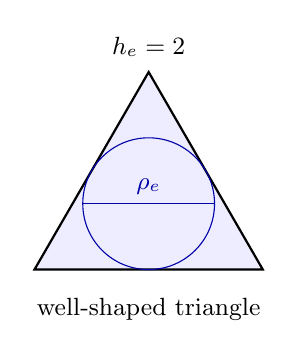
\begin{tikzpicture}[scale=1.45]
      \draw[thick,fill=blue!7] (-1,0)--(1,0)--(0,1.73)--cycle;
      \draw[blue!65!black] (0,0.577) circle[radius=0.577];
      \draw[blue!65!black] (-0.577,0.577)--(0.577,0.577);
      \node[font=\small,blue!65!black,above] at (0,0.577) {$\rho_e$};
      \node[font=\small] at (0,-0.35) {well-shaped triangle};
      \node[font=\small] at (0,1.95) {$h_e=2$};
    \end{tikzpicture}
  \end{column}
  \begin{column}{0.48\textwidth}
    \centering
    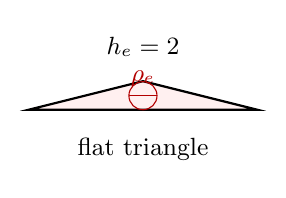
\begin{tikzpicture}[scale=1.45]
      \draw[thick,fill=red!6] (-1,0)--(1,0)--(0,0.25)--cycle;
      \draw[red!70!black] (0,0.123) circle[radius=0.123];
      \draw[red!70!black] (-0.123,0.123)--(0.123,0.123);
      \node[font=\small,red!70!black,above] at (0,0.123) {$\rho_e$};
      \node[font=\small] at (0,-0.35) {flat triangle};
      \node[font=\small] at (0,0.55) {$h_e=2$};
    \end{tikzpicture}
  \end{column}
\end{columns}
\vspace{0.2cm}
Both cells have the same diameter, but the diameter $\rho_e$ of the largest
inscribed disk is much smaller for the flat cell. The next two slides show
how this difference enters the affine element map and the basis-function
gradients.
\end{frame}

\begin{frame}{A family of affine triangles with the same diameter}
Let the reference triangle have vertices
\[
  \widehat\bx_1=(0,0),
  \qquad
  \widehat\bx_2=(1,0),
  \qquad
  \widehat\bx_3=(0,1).
\]
Map it to the physical triangle $\mathcal K_\varepsilon$ with vertices
\[
  \bx_1=(-1,0),
  \qquad
  \bx_2=(1,0),
  \qquad
  \bx_3=(0,\varepsilon),
\]
using
\[
  \bx=F_\varepsilon(\widehat\bx)
  =\bx_1+\bm J_\varepsilon\widehat\bx,
  \qquad
  \bm J_\varepsilon
  =
  \begin{bmatrix}
    2&1\\
    0&\varepsilon
  \end{bmatrix}.
\]
For $0<\varepsilon\leq\sqrt3$, the longest side is the base from $\bx_1$ to
$\bx_2$, so every triangle in this family has $h_e=2$. Decreasing
$\varepsilon$ changes the cell shape without changing its diameter.
\end{frame}

\begin{frame}{The inverse Jacobian amplifies a basis gradient}
The inverse transpose of the Jacobian is
\[
  \bm J_\varepsilon^{-T}
  =
  \begin{bmatrix}
    \tfrac12&0\\[2pt]
    -\tfrac{1}{2\varepsilon}&\tfrac{1}{\varepsilon}
  \end{bmatrix}.
\]
Choose the reference $P_1$ basis function associated with the third vertex:
\[
  \widehat v(\xi,\eta)=\eta,
  \qquad
  \nabla_{\widehat\bx}\widehat v=
  \begin{bmatrix}0\\1\end{bmatrix}.
\]
The gradient transformation from Chapter 6 gives
\[
  \nabla_{\bx}v
  =\bm J_\varepsilon^{-T}\nabla_{\widehat\bx}\widehat v
  =
  \begin{bmatrix}0\\1/\varepsilon\end{bmatrix},
  \qquad
  \norm{\nabla_{\bx}v}=\frac1\varepsilon.
\]
Thus $\norm{\bm J_\varepsilon^{-1}}\geq1/\varepsilon$. The basis gradient
remains moderate for $\varepsilon=\sqrt3$, but has magnitude $4$ when
$\varepsilon=1/4$.
\end{frame}

\begin{frame}{The same example gives the shape parameter}
The area of $\mathcal K_\varepsilon$ is $\varepsilon$, and its semiperimeter is
\[
  1+\sqrt{1+\varepsilon^2}.
\]
The radius of the inscribed disk is area divided by semiperimeter. Since
$\rho_e$ is the disk diameter,
\[
  \rho_e
  =\frac{2\varepsilon}{1+\sqrt{1+\varepsilon^2}},
  \qquad
  \frac{h_e}{\rho_e}
  =\frac{1+\sqrt{1+\varepsilon^2}}{\varepsilon}.
\]
As $\varepsilon\to0$,
\[
  \norm{\bm J_\varepsilon^{-1}}
  \text{ grows at least like }\frac1\varepsilon,
  \qquad
  \frac{h_e}{\rho_e}\text{ grows like }\frac2\varepsilon.
\]
The inverse-Jacobian factor is therefore controlled only when the cell-shape
ratio is controlled.
\end{frame}

\begin{frame}{Shape regularity}
For a cell $\mathcal K_e$:
\begin{itemize}
  \item $h_e=\operatorname{diam}(\mathcal K_e)$ is the largest distance
  between two points in the cell;
  \item $\rho_e$ is the diameter of the largest ball contained in the cell.
\end{itemize}
The ratio $h_e/\rho_e$ increases as a triangle or tetrahedron becomes flatter.

\vspace{0.25cm}
A family of meshes $\{\Th\}$ is \textbf{shape regular} if one constant
$\sigma$ satisfies
\[
  \boxed{\frac{h_e}{\rho_e}\leq\sigma}
  \qquad\text{for every cell in every mesh of the family.}
\]
Refinement may create smaller cells, but it may not create cells that become
progressively flatter.
\end{frame}

\begin{frame}{Local interpolation estimate}
The estimate is first obtained on the reference simplex and transferred to
$\mathcal K_e$ by the affine element map. Shape regularity keeps the
transformation constants independent of $h_e$.

Let $\Ih u$ be the degree-$p$ Lagrange interpolant. If
\[
  u\in H^s(\mathcal K_e),
  \qquad 2\leq s\leq p+1,
\]
then
\[
  \boxed{\norm[L^2(\mathcal K_e)]{u-\Ih u}
  \leq C_I h_e^s\seminorm[H^s(\mathcal K_e)]{u}}
\]
and
\[
  \boxed{\seminorm[H^1(\mathcal K_e)]{u-\Ih u}
  \leq C_I h_e^{s-1}\seminorm[H^s(\mathcal K_e)]{u}.}
\]
The constant $C_I$ is independent of $h_e$. It may depend on the polynomial
degree and on the common shape bound $\sigma$.
\end{frame}

\begin{frame}{From local interpolation error to global error}
The element interiors do not overlap, so
\[
  \norm[L^2(\Om)]{u-\Ih u}^2
  =\sum_e\norm[L^2(\mathcal K_e)]{u-\Ih u}^2.
\]
Using the local estimate and $h_e\leq h:=\max_eh_e$,
\begin{align*}
  \norm[L^2(\Om)]{u-\Ih u}^2
  &\leq C_I^2\sum_e h_e^{2s}\seminorm[H^s(\mathcal K_e)]{u}^2\\
  &\leq C_I^2h^{2s}\seminorm[H^s(\Om)]{u}^2.
\end{align*}
Therefore
\[
  \norm[L^2(\Om)]{u-\Ih u}\leq C_Ih^s\seminorm[H^s(\Om)]{u},
\]
and the same calculation gives
\[
  \seminorm[H^1(\Om)]{u-\Ih u}
  \leq C_Ih^{s-1}\seminorm[H^s(\Om)]{u}.
\]
\end{frame}

\begin{frame}{Key result from interpolation}
For a shape-regular family of affine simplicial meshes, degree-$p$ Lagrange
interpolation, and
\[
  u\in H^s(\Om),
  \qquad 2\leq s\leq p+1,
\]
the global estimates are
\[
  \boxed{
  \norm[L^2(\Om)]{u-\Ih u}
  \leq C_Ih^s\seminorm[H^s(\Om)]{u},}
\]
\[
  \boxed{
  \seminorm[H^1(\Om)]{u-\Ih u}
  \leq C_Ih^{s-1}\seminorm[H^s(\Om)]{u}.}
\]
For $h\leq1$, these two bounds also give
\[
  \norm[H^1(\Om)]{u-\Ih u}
  \leq \sqrt{2}\,C_Ih^{s-1}\seminorm[H^s(\Om)]{u}.
\]
The constant $C_I$ is independent of $h$.
\end{frame}

\section{Energy and \texorpdfstring{$H^1$}{H1} convergence}

\begin{frame}[plain]
  \centering
  \vfill
  {\LARGE\bfseries Finite element error estimates\par}
  \vspace{0.45cm}
  {\large Combine C\'ea's best-approximation result with the interpolation
  estimates.\par}
  \vfill
\end{frame}

\begin{frame}{C\'ea's lemma supplies the comparison}
The previous lecture proved C\'ea's estimate
\[
  \norm[V]{u-u_h}
  \leq \frac{M}{\alpha}
  \inf_{v_h\in\Vhzero}\norm[V]{u-v_h}.
\]
For symmetric diffusion, choose the energy norm. In this norm the
best-approximation constant is one, so
\[
  \norm[a]{u-u_h}
  \leq \norm[a]{u-v_h}
  \qquad\forall v_h\in\Vhzero.
\]
For homogeneous Dirichlet data on $\Gam_D$, with a mesh that resolves
$\Gam_D$, the interpolant satisfies $\Ih u\in\Vhzero$. Set
$v_h=\Ih u$:
\[
  \boxed{\norm[a]{u-u_h}\leq\norm[a]{u-\Ih u}.}
\]
\end{frame}

\begin{frame}{Energy-norm finite element error}
The coefficient bound $k(\bx)\leq k_1$ gives, for any $w\in\Vzero$,
\[
  \norm[a]{w}^2
  =\int_\Om k|\nabla w|^2\,\dd\bx
  \leq k_1\seminorm[H^1(\Om)]{w}^2.
\]
Set $w=u-\Ih u$ and use the two results in sequence:
\begin{align*}
  \norm[a]{u-u_h}
  &\leq \norm[a]{u-\Ih u}
    &&\text{(best approximation)}\\
  &\leq \sqrt{k_1}\seminorm[H^1(\Om)]{u-\Ih u}
    &&\text{(coefficient bound)}\\
  &\leq C_I\sqrt{k_1}\,h^{s-1}\seminorm[H^s(\Om)]{u}
    &&\text{(interpolation estimate).}
\end{align*}
Therefore
\[
  \boxed{\norm[a]{u-u_h}
  \leq C_I\sqrt{k_1}\,h^{s-1}\seminorm[H^s(\Om)]{u}.}
\]
\end{frame}

\begin{frame}{From energy error to \texorpdfstring{$H^1$}{H1} error}
For $v\in\Vzero$, Poincar\'e's inequality gives
\[
  \norm[H^1(\Om)]{v}^2
  =\norm[L^2(\Om)]{v}^2+\seminorm[H^1(\Om)]{v}^2
  \leq(1+C_P^2)\seminorm[H^1(\Om)]{v}^2.
\]
The lower coefficient bound gives
\[
  \norm[a]{v}^2
  =\int_\Om k|\nabla v|^2\,\dd\bx
  \geq k_0\seminorm[H^1(\Om)]{v}^2.
\]
Consequently,
\[
  \norm[H^1(\Om)]{v}
  \leq\sqrt{\frac{1+C_P^2}{k_0}}\norm[a]{v}.
\]
Set $v=u-u_h$ and substitute the energy estimate:
\[
  \boxed{\norm[H^1(\Om)]{u-u_h}
  \leq C_I\sqrt{\frac{k_1(1+C_P^2)}{k_0}}
  h^{s-1}\seminorm[H^s(\Om)]{u}.}
\]
\end{frame}

\begin{frame}{The \texorpdfstring{$L^2$}{L2} estimate and the remaining question}
With $e=u-u_h$,
\[
  \norm[L^2(\Om)]{e}
  \leq \norm[H^1(\Om)]{e}
  \leq C h^{s-1}\seminorm[H^s(\Om)]{u}.
\]
The argument used today therefore gives
\[
  \boxed{
  \norm[L^2(\Om)]{u-u_h}
  =O(h^{s-1}).}
\]
The $L^2$ interpolation estimate has one higher power of $h$:
\[
  \boxed{\norm[L^2(\Om)]{u-\Ih u}=O(h^s).}
\]
C\'ea's lemma controls the error in the energy norm, so it does not directly
transfer this $L^2$ interpolation estimate to $u-u_h$.

The duality argument developed in the next lecture provides the missing power
of $h$. We will prove
\[
  \boxed{\norm[L^2(\Om)]{u-u_h}\leq C h^s
  \seminorm[H^s(\Om)]{u}.}
\]
\end{frame}

\end{document}
